\section{\ara{} Verification and Review}
\label{sec:review-system}

Expert human attention is the scarcest resource in scientific evaluation.
Review loads at top venues have grown faster than the reviewer pool~\citep{aczel2021billiondollar}, and reviewer bandwidth is increasingly consumed by mechanical verification (``does the code run?'', ``does Table~3 support Claim~2?'') rather than the substantive judgment that only domain experts can provide.

Because an \ara{} submission \emph{is} a structured, machine-executable artifact, structural properties that PDF review checks subjectively become objectively verifiable: schema conformance and cross-layer reference integrity either pass or fail deterministically.
Higher-order properties, information completeness and directional reproducibility of central claims, become \emph{machine-assessable}: automated checks provide probabilistic evidence that informs human reviewers rather than replacing them.
This separation redirects expert attention from mechanical checking to the substantive judgment that only humans can provide: significance, novelty, and taste.
We define the \textbf{ARA Seal} as a machine-verifiable credential with three escalating levels (\S\ref{sec:liveness}, Figure~\ref{fig:ara-seal}) and describe a three-stage review pipeline (Figure~\ref{fig:review-pipeline}) that consumes those levels to separate automated verification from human judgment.

\subsection{Design Principles}
\label{sec:review-principles}

We derive two design principles below; cross-artifact review via agent-to-agent ARA comparison, which becomes meaningful only as the corpus reaches critical mass, is discussed in \S\ref{sec:discussion}.

\paragraph{P1. Automate the mechanical; reserve humans for judgment.}
Structural validity, internal consistency, and claim reproducibility are objective properties that either pass or fail, whereas significance, novelty, and taste require domain expertise.
The review system should never ask a human to verify that Experiment~E03 matches Claim~C02 when a machine can do so in seconds; resolving all machine-checkable issues \emph{before} the artifact reaches a human reviewer ensures that expert attention is spent exclusively on questions that genuinely require it.

\paragraph{P2. Reproducibility as a foundational requirement.}
``Code available upon request'' nominally satisfies today's reproducibility bar; in an \ara{}-native system, reproducibility is a \emph{machine-verified property} of the artifact itself.
Passing ARA Seal Level~1 (structural integrity) is a submission requirement, and Level~2 (argumentative rigor) produces a structured critique before the venue spends compute on Level~3 (execution reproducibility), whose results are then attached to every review.
Artifacts that fail structural checks, or whose claims remain obviously under-supported after Level~2 critique, do not advance to human review.

\subsection{The ARA Seal: Machine-Verifiable Research Credentials}
\label{sec:liveness}

\begin{figure}[!t]
    \centering
    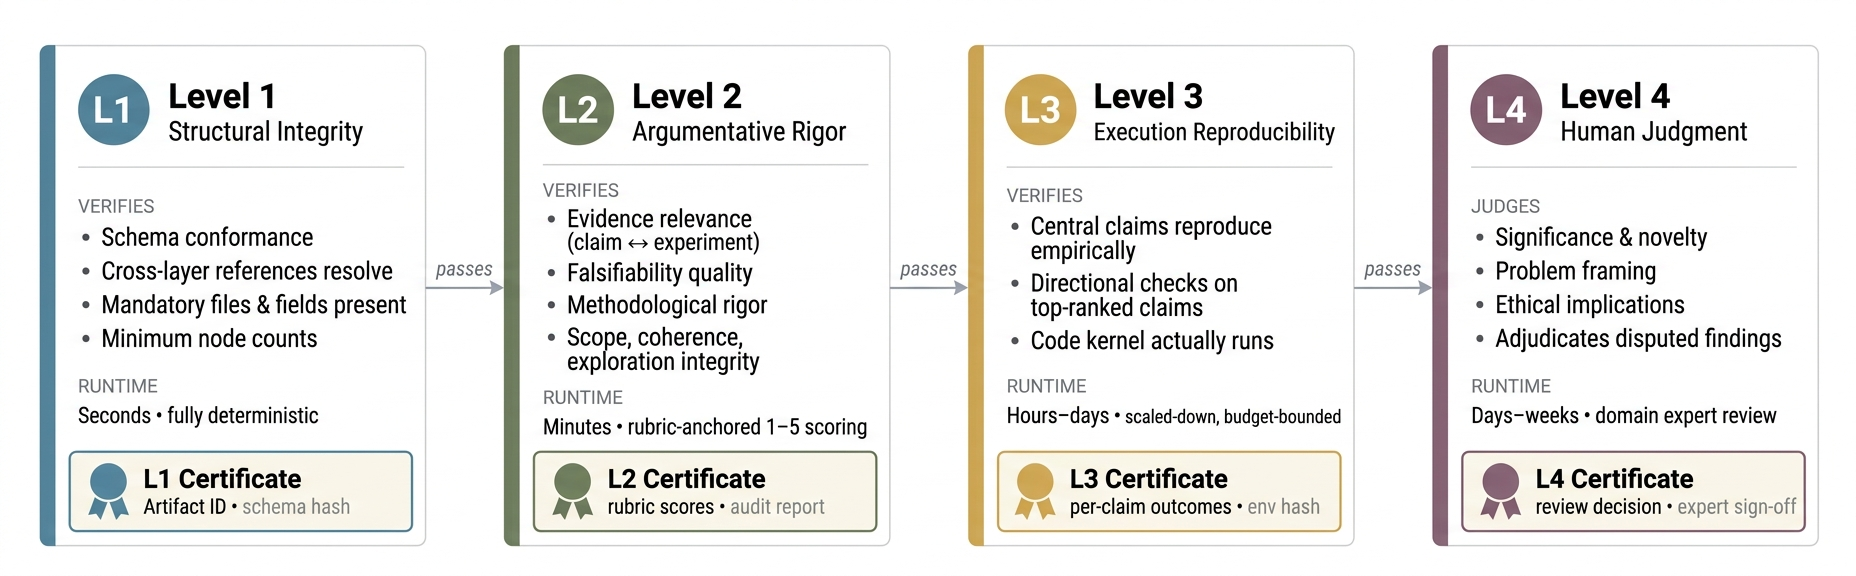
\includegraphics[width=\linewidth]{figures/fig_ara_seal.png}
    \caption{The ARA Seal is a three-level verification credential. Each level tests a progressively stronger property of the artifact, escalating in cost and breadth: structural integrity (seconds, deterministic), argumentative rigor (minutes, rubric-anchored agent), and execution reproducibility (hours to days, sandboxed coding agent). Passing the applicable levels issues a Seal Certificate that downstream agents check before investing compute.}
    \label{fig:ara-seal}
\end{figure}

A PDF paper earns trust indirectly: venue prestige, citation counts, and author reputation serve as proxies for quality, but none verify the work itself.
Because an \ara{} encodes research as typed, machine-traversable data with explicit claim--evidence bindings, its quality becomes \emph{directly verifiable}.
The ARA Seal operationalizes this as a three-level verification protocol (Figure~\ref{fig:ara-seal}), where each level tests a progressively stronger property (implementation details in Appendix~\ref{app:seal-details}).

\begin{description}[leftmargin=1.5em, itemsep=4pt, topsep=2pt]
    \item[Level 1 -- Structural Integrity]
    verifies that the artifact is well-formed and internally consistent:
    the directory ontology exists, all structured files conform to their schema (each claim carries \texttt{Statement}, \texttt{Status}, \texttt{Falsification criteria}, and \texttt{Proof}; each heuristic carries \texttt{Rationale}, \texttt{Sensitivity}, and \texttt{Bounds}),
    and all cross-layer references resolve (experiment IDs in \texttt{claims.md} point to valid entries in \texttt{experiments.md}, code references trace to implementations in \texttt{/src}).

    
    \item[Level 2 -- Argumentative Rigor]
    without executing any code or consulting external sources, a \emph{Rigor Auditor} agent evaluates whether the content of a Level-1-valid artifact is epistemically sound along six objective dimensions, each scored on an anchored 1 to 5 rubric.
    The three load-bearing dimensions are:
    \emph{evidence relevance}, checking that every claim's cited experiments substantively address what the claim asserts under type-aware entailment (causal claims require isolating ablations, generalization claims require heterogeneous test conditions, improvement claims require baseline comparisons);
    \emph{falsifiability quality}, checking that criteria are actionable, non-tautological, scope-matched, and independently testable without access to proprietary data;
    and \emph{methodological rigor}, covering baseline adequacy, ablation coverage, statistical reporting, and metric--claim alignment.
    Three further dimensions---scope calibration, argument coherence, and exploration integrity---are defined in Appendix~\ref{app:seal-eval-l2}.
    Findings are collected with severity (\emph{critical}, \emph{major}, \emph{minor}, \emph{suggestion}), verbatim evidence spans, and actionable suggestions; the overall grade is derived from the mean score and per-dimension floors.
    Every check reduces to a rubric-anchored property of the artifact's content, so Level~2 remains objective; judgments of significance, novelty, and taste are reserved for human reviewers in Stage~3.
    The reference Rigor Auditor is released as an agent skill~\citep{agentskills2025};\footnote{\url{github.com/AmberLJC/Agent-Native-Research-Artifact}} full protocol, dimension rubrics, and grade thresholds appear in Appendix~\ref{app:seal-eval-l2}.

    \item[Level 3 -- Execution Reproducibility]
    verifies that the artifact's central claims reproduce empirically.
    The system selects claims by criticality---those in the contribution list, those anchoring the most downstream dependencies, or those flagged by the authors---and runs scaled-down directional checks (small data, few epochs, toy configurations) that test whether claimed properties hold qualitatively rather than reproducing exact numbers.
    The verifying agent is isolated from the artifact's evidence layer: it receives only the code kernel and algorithm descriptions, never the reported numbers, preventing fabrication by copying expected outcomes.
    Venues set a compute budget; claims that exceed it are flagged as \emph{unverified}.
    Full-scale reproduction (original datasets, full training runs, exact metric recovery) is optional and typically post-acceptance or community-driven; results are appended to the living Seal certificate.
\end{description}

Passing the applicable levels issues a \textbf{Seal Certificate}---a signed record of artifact ID, verification level achieved, timestamp, environment hash, and per-claim reproduction outcomes.
Downstream agents check this certificate before investing compute, avoiding redundant re-verification.


\subsection{Three-Stage Review Pipeline}

\begin{figure}[!t]
    \centering
    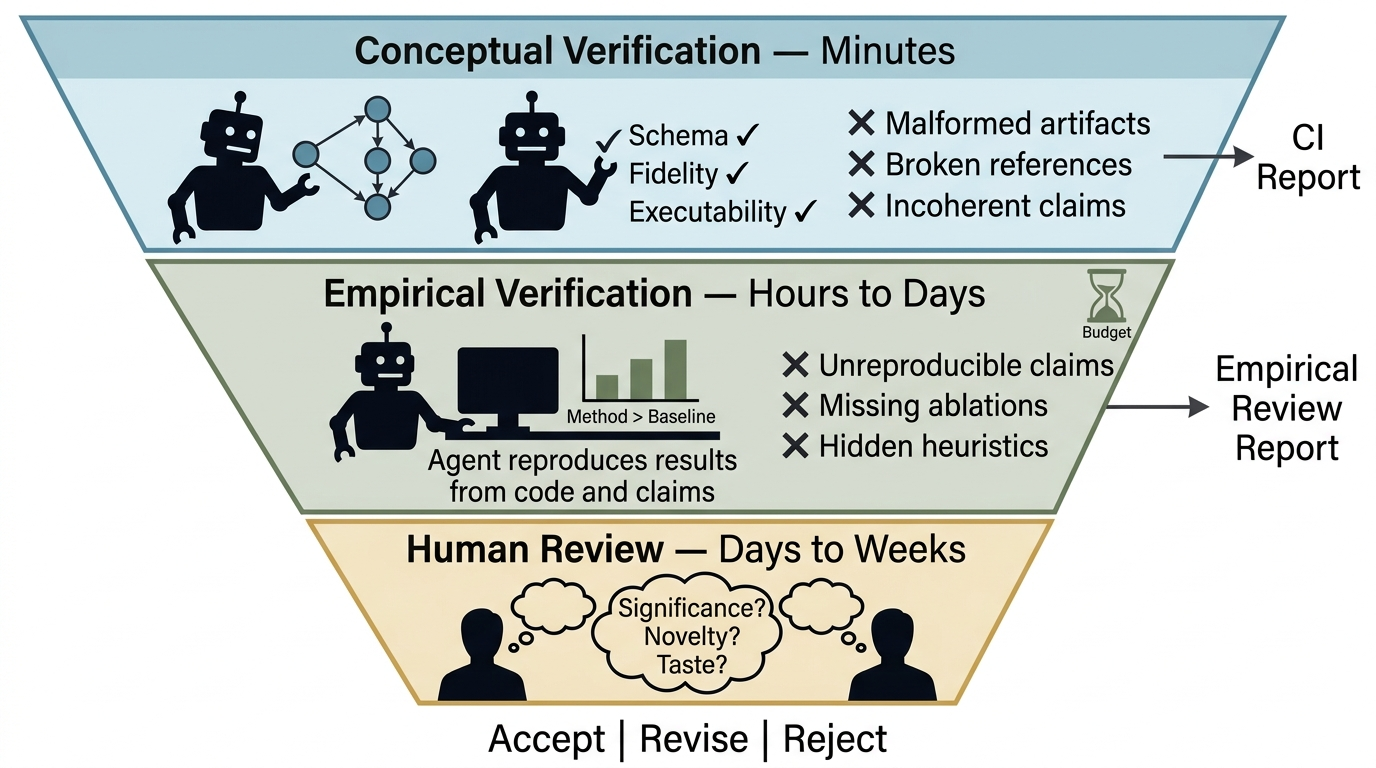
\includegraphics[width=\linewidth]{figures/fig_review_pipeline_v2.png}
    \caption{Three-stage \ara{}-native review pipeline. Stages~1--2 invoke the ARA Seal levels of Figure~\ref{fig:ara-seal} to resolve mechanical and rigor issues before human reviewers engage, redirecting expert attention to novelty and significance.}
    \label{fig:review-pipeline}
\end{figure}

We envision a three-stage review pipeline (Figure~\ref{fig:review-pipeline}) that mirrors CI/CD practices, where each stage gates the next: conceptual verification, empirical verification, and human judgment.

\paragraph{Stage 1: Conceptual Verification (Minutes).}
The first stage checks whether the artifact is \emph{well-formed and conceptually well-supported} without running any experiments.
Automated checks validate structural integrity (ARA Seal Level~1---schema conformance, cross-layer reference resolution, required field completeness), and the Rigor Auditor executes Level~2 argumentative rigor by assessing whether major claims are appropriately scoped, whether attached evidence and ablations justify them, and whether obvious baselines, assumptions, or limitations are missing.
Level~1 checks are mechanical and deterministic: either every claim in \texttt{claims.md} links to a valid experiment, or it does not; either heuristics carry sensitivity bounds, or they are missing.
Level~2 instead produces a structured rigor report keyed to specific claims, experiments, and omissions.
The stage also generates \emph{advisory diagnostics} surfaced to human reviewers in Stage~3: whether the exploration tree contains dead-end nodes (suggesting genuine process documentation versus a sanitized linear chain), whether the related-work graph covers obvious baselines, and whether experiment--claim coverage has gaps.
These diagnostics inform but do not gate; only the Seal checks are pass/fail requirements.
The output is a \textbf{CI Report} plus a Level~2 rigor report, both attached to the submission and visible to authors and reviewers.
Authors iterate on structural failures and rigor critiques before the artifact advances, analogous to fixing lint errors and design issues before code review.

\paragraph{Stage 2: Empirical Verification (Hours--Days).}
Once the artifact passes conceptual review, the second stage tests whether the \emph{claimed results actually reproduce}.
An AI reviewer agent executes ARA Seal Level~3: it ranks the artifact's claims by criticality---prioritizing those in the contribution list and those with the most downstream dependents in the claim graph---then runs scaled-down directional checks (small data, few epochs, toy configurations) within a venue-specified compute budget.
The agent is isolated from the artifact's evidence layer and ground-truth results: it receives only the code kernel and algorithm descriptions, never the paper's reported numbers, preventing fabrication by copying expected outcomes.
For each tested claim, it reports whether the claimed direction holds (e.g., ``method A outperforms baseline B on metric M''), wall-clock time consumed, and any divergence from expected outcomes.
Claims that exceed the remaining budget are flagged as \emph{unverified} with an estimate of the compute required.
Beyond reproduction, the agent assesses experimental comprehensiveness: Are ablations present for each design choice?
Do the experimental conditions cover the claimed generality, or are results cherry-picked from favorable settings?
Are there undocumented heuristics in the code that do not appear in the artifact's cognitive layer?
The output is an \textbf{Empirical Review Report} that records which claims were verified, which failed, which were deferred due to budget, and what experimental gaps were identified.

\paragraph{Stage 3: Human Review (Days--Weeks).}
Human reviewers receive the submission alongside the CI Report and Empirical Review Report, and their role shifts from \emph{verification}---already handled by Stages~1--2---to \emph{judgment}.
They focus on the questions that no machine can answer: Is this contribution significant---does it address a real problem that matters?
Is the core insight genuinely novel, or an incremental recombination of known ideas?
Is this the right formulation of the problem, and are there better approaches the authors should have considered?
What are the ethical implications and potential for misuse?
Where the AI reviewer's findings are contested by the authors, humans adjudicate with the full audit trail available for inspection.
Human reviewers write structured reviews in the same typed format---findings linked to specific \ara{} components---ensuring that all feedback is actionable and traceable.
The key efficiency gain: humans no longer spend time on ``your code doesn't run'' or ``Table~3 contradicts Claim~2''---these are resolved before the artifact reaches them.
